\chapter{Budget and Timeline Summary}
% Give a summary of actual and anticipated purchases (include shipping and
% delivery). to met s and results are encouraged, regardless of success. A
% timeline summary from start of the project to completion should be included –
% a Gantt chart may be appropriate.

\section{Budget}
After building preliminary system designs, a bill of materials including parts
costs has been composed. Where possible pieces have been from either Digikey,
Element 14, Mouser or estimated if the components will come from the ECE store.

Currently both the Gear Motor with Encoder and the Linear actuator have been
ordered as they have a month lead time coming from the USA. All other components
will be ordered within the next two weeks.

{\small
\begin{tabular}{ | l | l | p{.40\textwidth} | l | l | l | l | }
\hline
 & Part Number & Description & Qty & Cost & Subtotal \\
\hline
\multirow{4}{*}{Steering} & IG52 – 04 & 24VDC 10rpm Gear Motor with Encoder & 1 & \$185.00 & \$185.00 \\
 & Shipping & Gear Motor Shipping & 1 & \$75.00 & \$75.00 \\
 &  & Motor Driver & 1 & \$0.00 & \$0.00 \\
 &  & Mounting Bracket & 1 & \$50.00 & \$50.00 \\
\hline
\multirow{4}{*}{Breaking} & 5 1752 & 4 inch stroke 100lb 24VDC Linear actuator  & 1 & \$50.00 & \$50.00 \\
 & Shipping & Linear actuator Shipping & 1 & \$50.00 & \$50.00 \\
 &  & Mounting Bracket & 1 & \$50.00 & \$50.00 \\
\hline
\multirow{3}{*}{Accelerator} & ATMEGA8L & Interface to go-kart power control & 1 & \$5.16 & \$5.16 \\
 & LM317KCS & IC VOLT REG POS ADJ & 1 & \$1.13 & \$1.13 \\
 &  & PCB & 1 & \$20.00 & \$20.00 \\
\hline
\multirow{11}{*}{CAN Bus} & PL-STP6-0 & 0.5M Cat6 STP Lead (CAN Bus) & 3 & \$4.50 & \$13.50 \\
 & PL-STP6-1 & 1.0M Cat6 STP Lead (CAN Bus) & 1 & \$5.70 & \$5.70 \\
 & SS60000-009G & RJ45 JACK (CAN Input/output) & 10 & \$4.96 & \$49.60 \\
 & Header 10X2 & Header, 10-Pin, Dual row (JTAG ) & 5 & \$1.00 & \$5.00 \\
 & fdd8445 & MOSFET 40V, 50A, 8.7mΩ & 5 & \$2.00 & \$10.00 \\
 & SW-PB & Switch (Reset) & 5 & \$3.00 & \$15.00 \\
 & AT91SAM7X & Microcontroller (CAN Controller) & 5 & \$19.37 & \$96.85 \\
 & ATA6660 & High Speed CAN Transceiver & 5 & \$2.47 & \$12.35 \\
 & AE9925-ND & USB Type B connector & 5 & \$1.52 & \$7.60 \\
 & MCP130T-300I & Microcontroller Supervisory Circuit & 5 & \$0.76 & \$3.80 \\
 &  & PCB Manufacture and shipping & 1 & \$217.00 & \$217.00 \\
\hline
\multirow{4}{*}{Other} &  & Misc Components (Diodes, Resistors, Capacitors, Wire, Headers) & 1 & \$60.00 & \$60.00 \\
 & Shipping & Shipping from Digikey and Element14 & 1 & \$30.00 & \$30.00 \\
\hline
 &  &  &  & Total & \$1,012.69 \\
\hline
\end{tabular}
}



\section{Timeline}
The Autonomous Go-Kart project has been broken down into small sections then time
allocations have been put next to each task. Where possible we have put in
dependencies between each of the tasks. However this model of only starting one
task once the previous one has been completed is not very accurate. For example
the control software has been represented as requiring the hardware to be
complete. Actually the control software will be started much before the hardware
is complete.

To make sure the project deadlines are met, milestones have been added for each
assessment or hand in item. 

%if we are on track
%Second section of Autonomous work and how it pushes past hand in


  \begin{figure}[h]
    \centering
    %\includegraphics[width=0.5\textwidth]{Images/TB9100.jpg}
    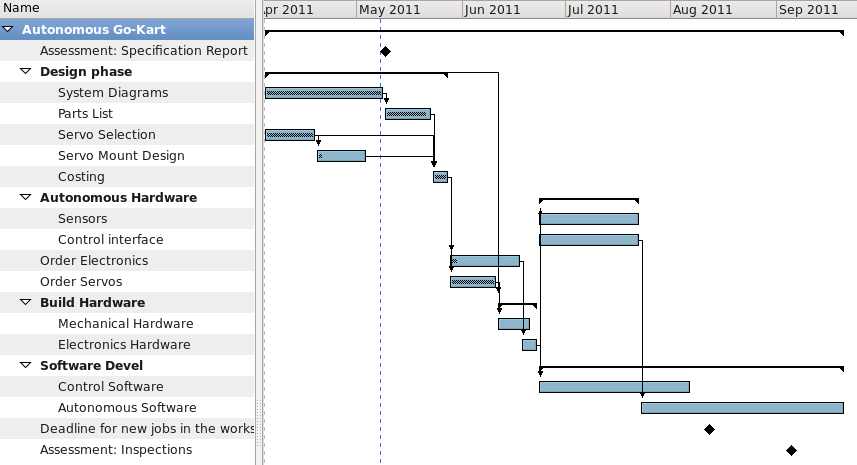
\includegraphics[width=1.0\textwidth]{Images/Gantt.png}
    \caption{Gantt chart of the Autonomous Go-Kart project}
    \label{gantt_chart}
  \end{figure}
